% Created by tikzDevice version 0.12.3.1 on 2022-05-11 23:33:04
% !TEX encoding = UTF-8 Unicode
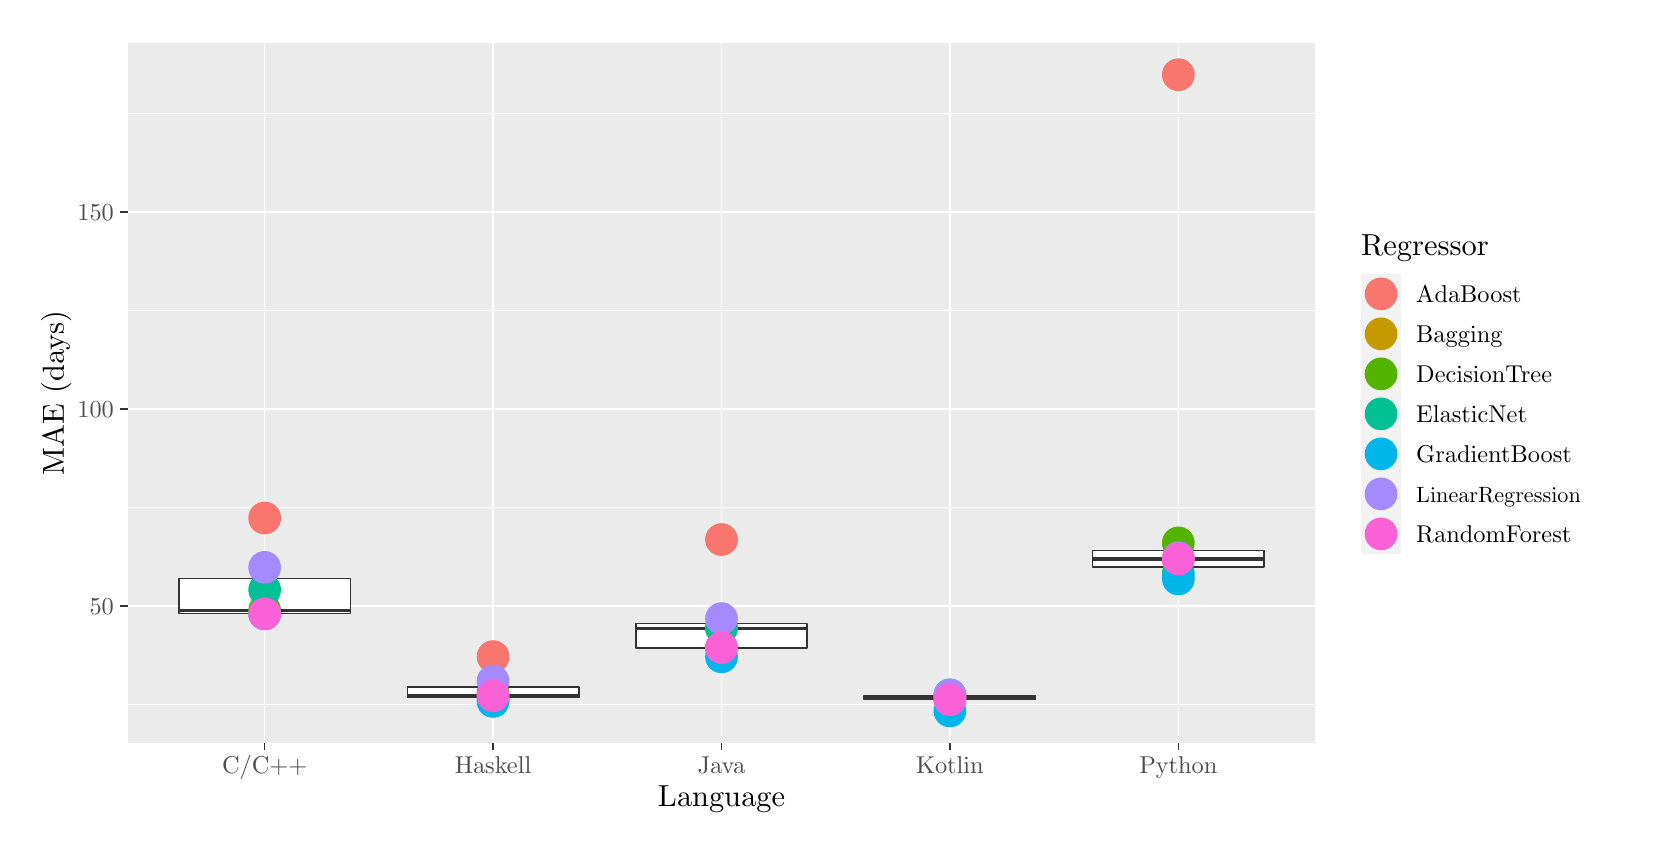
\begin{tikzpicture}[x=1pt,y=1pt]
\definecolor{fillColor}{RGB}{255,255,255}
\path[use as bounding box,fill=fillColor,fill opacity=0.00] (0,0) rectangle (578.16,289.08);
\begin{scope}
\path[clip] (  0.00,  0.00) rectangle (578.16,289.08);
\definecolor{drawColor}{RGB}{255,255,255}
\definecolor{fillColor}{RGB}{255,255,255}

\path[draw=drawColor,line width= 0.6pt,line join=round,line cap=round,fill=fillColor] (  0.00,  0.00) rectangle (578.16,289.08);
\end{scope}
\begin{scope}
\path[clip] ( 36.11, 30.69) rectangle (465.31,283.58);
\definecolor{fillColor}{gray}{0.92}

\path[fill=fillColor] ( 36.11, 30.69) rectangle (465.31,283.58);
\definecolor{drawColor}{RGB}{255,255,255}

\path[draw=drawColor,line width= 0.3pt,line join=round] ( 36.11, 44.41) --
	(465.31, 44.41);

\path[draw=drawColor,line width= 0.3pt,line join=round] ( 36.11,115.62) --
	(465.31,115.62);

\path[draw=drawColor,line width= 0.3pt,line join=round] ( 36.11,186.82) --
	(465.31,186.82);

\path[draw=drawColor,line width= 0.3pt,line join=round] ( 36.11,258.02) --
	(465.31,258.02);

\path[draw=drawColor,line width= 0.6pt,line join=round] ( 36.11, 80.01) --
	(465.31, 80.01);

\path[draw=drawColor,line width= 0.6pt,line join=round] ( 36.11,151.22) --
	(465.31,151.22);

\path[draw=drawColor,line width= 0.6pt,line join=round] ( 36.11,222.42) --
	(465.31,222.42);

\path[draw=drawColor,line width= 0.6pt,line join=round] ( 85.63, 30.69) --
	( 85.63,283.58);

\path[draw=drawColor,line width= 0.6pt,line join=round] (168.17, 30.69) --
	(168.17,283.58);

\path[draw=drawColor,line width= 0.6pt,line join=round] (250.71, 30.69) --
	(250.71,283.58);

\path[draw=drawColor,line width= 0.6pt,line join=round] (333.25, 30.69) --
	(333.25,283.58);

\path[draw=drawColor,line width= 0.6pt,line join=round] (415.79, 30.69) --
	(415.79,283.58);
\definecolor{drawColor}{gray}{0.20}
\definecolor{fillColor}{gray}{0.20}

\path[draw=drawColor,line width= 0.4pt,line join=round,line cap=round,fill=fillColor] ( 85.63,111.89) circle (  1.96);

\path[draw=drawColor,line width= 0.6pt,line join=round] ( 85.63, 90.02) -- ( 85.63, 94.06);

\path[draw=drawColor,line width= 0.6pt,line join=round] ( 85.63, 77.34) -- ( 85.63, 77.25);
\definecolor{fillColor}{RGB}{255,255,255}

\path[draw=drawColor,line width= 0.6pt,line join=round,line cap=round,fill=fillColor] ( 54.68, 90.02) --
	( 54.68, 77.34) --
	(116.59, 77.34) --
	(116.59, 90.02) --
	( 54.68, 90.02) --
	cycle;

\path[draw=drawColor,line width= 1.1pt,line join=round] ( 54.68, 78.61) -- (116.59, 78.61);
\definecolor{fillColor}{gray}{0.20}

\path[draw=drawColor,line width= 0.4pt,line join=round,line cap=round,fill=fillColor] (168.17, 61.81) circle (  1.96);

\path[draw=drawColor,line width= 0.6pt,line join=round] (168.17, 50.81) -- (168.17, 52.97);

\path[draw=drawColor,line width= 0.6pt,line join=round] (168.17, 47.07) -- (168.17, 45.62);
\definecolor{fillColor}{RGB}{255,255,255}

\path[draw=drawColor,line width= 0.6pt,line join=round,line cap=round,fill=fillColor] (137.22, 50.81) --
	(137.22, 47.07) --
	(199.12, 47.07) --
	(199.12, 50.81) --
	(137.22, 50.81) --
	cycle;

\path[draw=drawColor,line width= 1.1pt,line join=round] (137.22, 47.77) -- (199.12, 47.77);
\definecolor{fillColor}{gray}{0.20}

\path[draw=drawColor,line width= 0.4pt,line join=round,line cap=round,fill=fillColor] (250.71,104.11) circle (  1.96);

\path[draw=drawColor,line width= 0.6pt,line join=round] (250.71, 73.83) -- (250.71, 75.55);

\path[draw=drawColor,line width= 0.6pt,line join=round] (250.71, 65.00) -- (250.71, 61.73);
\definecolor{fillColor}{RGB}{255,255,255}

\path[draw=drawColor,line width= 0.6pt,line join=round,line cap=round,fill=fillColor] (219.76, 73.83) --
	(219.76, 65.00) --
	(281.66, 65.00) --
	(281.66, 73.83) --
	(219.76, 73.83) --
	cycle;

\path[draw=drawColor,line width= 1.1pt,line join=round] (219.76, 72.11) -- (281.66, 72.11);
\definecolor{fillColor}{gray}{0.20}

\path[draw=drawColor,line width= 0.4pt,line join=round,line cap=round,fill=fillColor] (333.25, 42.18) circle (  1.96);

\path[draw=drawColor,line width= 0.6pt,line join=round] (333.25, 47.66) -- (333.25, 47.97);

\path[draw=drawColor,line width= 0.6pt,line join=round] (333.25, 46.30) -- (333.25, 46.25);
\definecolor{fillColor}{RGB}{255,255,255}

\path[draw=drawColor,line width= 0.6pt,line join=round,line cap=round,fill=fillColor] (302.30, 47.66) --
	(302.30, 46.30) --
	(364.20, 46.30) --
	(364.20, 47.66) --
	(302.30, 47.66) --
	cycle;

\path[draw=drawColor,line width= 1.1pt,line join=round] (302.30, 46.53) -- (364.20, 46.53);
\definecolor{fillColor}{gray}{0.20}

\path[draw=drawColor,line width= 0.4pt,line join=round,line cap=round,fill=fillColor] (415.79,272.08) circle (  1.96);

\path[draw=drawColor,line width= 0.6pt,line join=round] (415.79,100.21) -- (415.79,102.90);

\path[draw=drawColor,line width= 0.6pt,line join=round] (415.79, 94.29) -- (415.79, 89.89);
\definecolor{fillColor}{RGB}{255,255,255}

\path[draw=drawColor,line width= 0.6pt,line join=round,line cap=round,fill=fillColor] (384.83,100.21) --
	(384.83, 94.29) --
	(446.74, 94.29) --
	(446.74,100.21) --
	(384.83,100.21) --
	cycle;

\path[draw=drawColor,line width= 1.1pt,line join=round] (384.83, 97.08) -- (446.74, 97.08);
\definecolor{drawColor}{RGB}{248,118,109}
\definecolor{fillColor}{RGB}{248,118,109}

\path[draw=drawColor,line width= 0.4pt,line join=round,line cap=round,fill=fillColor] ( 85.63,111.89) circle (  5.71);
\definecolor{drawColor}{RGB}{196,154,0}
\definecolor{fillColor}{RGB}{196,154,0}

\path[draw=drawColor,line width= 0.4pt,line join=round,line cap=round,fill=fillColor] ( 85.63, 77.43) circle (  5.71);
\definecolor{drawColor}{RGB}{83,180,0}
\definecolor{fillColor}{RGB}{83,180,0}

\path[draw=drawColor,line width= 0.4pt,line join=round,line cap=round,fill=fillColor] ( 85.63, 78.61) circle (  5.71);
\definecolor{drawColor}{RGB}{0,192,148}
\definecolor{fillColor}{RGB}{0,192,148}

\path[draw=drawColor,line width= 0.4pt,line join=round,line cap=round,fill=fillColor] ( 85.63, 85.98) circle (  5.71);
\definecolor{drawColor}{RGB}{0,182,235}
\definecolor{fillColor}{RGB}{0,182,235}

\path[draw=drawColor,line width= 0.4pt,line join=round,line cap=round,fill=fillColor] ( 85.63, 77.26) circle (  5.71);
\definecolor{drawColor}{RGB}{165,138,255}
\definecolor{fillColor}{RGB}{165,138,255}

\path[draw=drawColor,line width= 0.4pt,line join=round,line cap=round,fill=fillColor] ( 85.63, 94.06) circle (  5.71);
\definecolor{drawColor}{RGB}{251,97,215}
\definecolor{fillColor}{RGB}{251,97,215}

\path[draw=drawColor,line width= 0.4pt,line join=round,line cap=round,fill=fillColor] ( 85.63, 77.25) circle (  5.71);
\definecolor{drawColor}{RGB}{248,118,109}
\definecolor{fillColor}{RGB}{248,118,109}

\path[draw=drawColor,line width= 0.4pt,line join=round,line cap=round,fill=fillColor] (168.17, 61.81) circle (  5.71);
\definecolor{drawColor}{RGB}{196,154,0}
\definecolor{fillColor}{RGB}{196,154,0}

\path[draw=drawColor,line width= 0.4pt,line join=round,line cap=round,fill=fillColor] (168.17, 47.77) circle (  5.71);
\definecolor{drawColor}{RGB}{83,180,0}
\definecolor{fillColor}{RGB}{83,180,0}

\path[draw=drawColor,line width= 0.4pt,line join=round,line cap=round,fill=fillColor] (168.17, 48.65) circle (  5.71);
\definecolor{drawColor}{RGB}{0,192,148}
\definecolor{fillColor}{RGB}{0,192,148}

\path[draw=drawColor,line width= 0.4pt,line join=round,line cap=round,fill=fillColor] (168.17, 46.51) circle (  5.71);
\definecolor{drawColor}{RGB}{0,182,235}
\definecolor{fillColor}{RGB}{0,182,235}

\path[draw=drawColor,line width= 0.4pt,line join=round,line cap=round,fill=fillColor] (168.17, 45.62) circle (  5.71);
\definecolor{drawColor}{RGB}{165,138,255}
\definecolor{fillColor}{RGB}{165,138,255}

\path[draw=drawColor,line width= 0.4pt,line join=round,line cap=round,fill=fillColor] (168.17, 52.97) circle (  5.71);
\definecolor{drawColor}{RGB}{251,97,215}
\definecolor{fillColor}{RGB}{251,97,215}

\path[draw=drawColor,line width= 0.4pt,line join=round,line cap=round,fill=fillColor] (168.17, 47.63) circle (  5.71);
\definecolor{drawColor}{RGB}{248,118,109}
\definecolor{fillColor}{RGB}{248,118,109}

\path[draw=drawColor,line width= 0.4pt,line join=round,line cap=round,fill=fillColor] (250.71,104.11) circle (  5.71);
\definecolor{drawColor}{RGB}{196,154,0}
\definecolor{fillColor}{RGB}{196,154,0}

\path[draw=drawColor,line width= 0.4pt,line join=round,line cap=round,fill=fillColor] (250.71, 64.94) circle (  5.71);
\definecolor{drawColor}{RGB}{83,180,0}
\definecolor{fillColor}{RGB}{83,180,0}

\path[draw=drawColor,line width= 0.4pt,line join=round,line cap=round,fill=fillColor] (250.71, 72.11) circle (  5.71);
\definecolor{drawColor}{RGB}{0,192,148}
\definecolor{fillColor}{RGB}{0,192,148}

\path[draw=drawColor,line width= 0.4pt,line join=round,line cap=round,fill=fillColor] (250.71, 72.11) circle (  5.71);
\definecolor{drawColor}{RGB}{0,182,235}
\definecolor{fillColor}{RGB}{0,182,235}

\path[draw=drawColor,line width= 0.4pt,line join=round,line cap=round,fill=fillColor] (250.71, 61.73) circle (  5.71);
\definecolor{drawColor}{RGB}{165,138,255}
\definecolor{fillColor}{RGB}{165,138,255}

\path[draw=drawColor,line width= 0.4pt,line join=round,line cap=round,fill=fillColor] (250.71, 75.55) circle (  5.71);
\definecolor{drawColor}{RGB}{251,97,215}
\definecolor{fillColor}{RGB}{251,97,215}

\path[draw=drawColor,line width= 0.4pt,line join=round,line cap=round,fill=fillColor] (250.71, 65.06) circle (  5.71);
\definecolor{drawColor}{RGB}{248,118,109}
\definecolor{fillColor}{RGB}{248,118,109}

\path[draw=drawColor,line width= 0.4pt,line join=round,line cap=round,fill=fillColor] (333.25, 47.36) circle (  5.71);
\definecolor{drawColor}{RGB}{196,154,0}
\definecolor{fillColor}{RGB}{196,154,0}

\path[draw=drawColor,line width= 0.4pt,line join=round,line cap=round,fill=fillColor] (333.25, 46.35) circle (  5.71);
\definecolor{drawColor}{RGB}{83,180,0}
\definecolor{fillColor}{RGB}{83,180,0}

\path[draw=drawColor,line width= 0.4pt,line join=round,line cap=round,fill=fillColor] (333.25, 46.53) circle (  5.71);
\definecolor{drawColor}{RGB}{0,192,148}
\definecolor{fillColor}{RGB}{0,192,148}

\path[draw=drawColor,line width= 0.4pt,line join=round,line cap=round,fill=fillColor] (333.25, 47.97) circle (  5.71);
\definecolor{drawColor}{RGB}{0,182,235}
\definecolor{fillColor}{RGB}{0,182,235}

\path[draw=drawColor,line width= 0.4pt,line join=round,line cap=round,fill=fillColor] (333.25, 42.18) circle (  5.71);
\definecolor{drawColor}{RGB}{165,138,255}
\definecolor{fillColor}{RGB}{165,138,255}

\path[draw=drawColor,line width= 0.4pt,line join=round,line cap=round,fill=fillColor] (333.25, 47.96) circle (  5.71);
\definecolor{drawColor}{RGB}{251,97,215}
\definecolor{fillColor}{RGB}{251,97,215}

\path[draw=drawColor,line width= 0.4pt,line join=round,line cap=round,fill=fillColor] (333.25, 46.25) circle (  5.71);
\definecolor{drawColor}{RGB}{248,118,109}
\definecolor{fillColor}{RGB}{248,118,109}

\path[draw=drawColor,line width= 0.4pt,line join=round,line cap=round,fill=fillColor] (415.79,272.08) circle (  5.71);
\definecolor{drawColor}{RGB}{196,154,0}
\definecolor{fillColor}{RGB}{196,154,0}

\path[draw=drawColor,line width= 0.4pt,line join=round,line cap=round,fill=fillColor] (415.79, 96.76) circle (  5.71);
\definecolor{drawColor}{RGB}{83,180,0}
\definecolor{fillColor}{RGB}{83,180,0}

\path[draw=drawColor,line width= 0.4pt,line join=round,line cap=round,fill=fillColor] (415.79,102.90) circle (  5.71);
\definecolor{drawColor}{RGB}{0,192,148}
\definecolor{fillColor}{RGB}{0,192,148}

\path[draw=drawColor,line width= 0.4pt,line join=round,line cap=round,fill=fillColor] (415.79, 91.82) circle (  5.71);
\definecolor{drawColor}{RGB}{0,182,235}
\definecolor{fillColor}{RGB}{0,182,235}

\path[draw=drawColor,line width= 0.4pt,line join=round,line cap=round,fill=fillColor] (415.79, 89.89) circle (  5.71);
\definecolor{drawColor}{RGB}{165,138,255}
\definecolor{fillColor}{RGB}{165,138,255}

\path[draw=drawColor,line width= 0.4pt,line join=round,line cap=round,fill=fillColor] (415.79, 97.52) circle (  5.71);
\definecolor{drawColor}{RGB}{251,97,215}
\definecolor{fillColor}{RGB}{251,97,215}

\path[draw=drawColor,line width= 0.4pt,line join=round,line cap=round,fill=fillColor] (415.79, 97.08) circle (  5.71);
\end{scope}
\begin{scope}
\path[clip] (  0.00,  0.00) rectangle (578.16,289.08);
\definecolor{drawColor}{gray}{0.30}

\node[text=drawColor,anchor=base east,inner sep=0pt, outer sep=0pt, scale=  0.88] at ( 31.16, 76.98) {50};

\node[text=drawColor,anchor=base east,inner sep=0pt, outer sep=0pt, scale=  0.88] at ( 31.16,148.19) {100};

\node[text=drawColor,anchor=base east,inner sep=0pt, outer sep=0pt, scale=  0.88] at ( 31.16,219.39) {150};
\end{scope}
\begin{scope}
\path[clip] (  0.00,  0.00) rectangle (578.16,289.08);
\definecolor{drawColor}{gray}{0.20}

\path[draw=drawColor,line width= 0.6pt,line join=round] ( 33.36, 80.01) --
	( 36.11, 80.01);

\path[draw=drawColor,line width= 0.6pt,line join=round] ( 33.36,151.22) --
	( 36.11,151.22);

\path[draw=drawColor,line width= 0.6pt,line join=round] ( 33.36,222.42) --
	( 36.11,222.42);
\end{scope}
\begin{scope}
\path[clip] (  0.00,  0.00) rectangle (578.16,289.08);
\definecolor{drawColor}{gray}{0.20}

\path[draw=drawColor,line width= 0.6pt,line join=round] ( 85.63, 27.94) --
	( 85.63, 30.69);

\path[draw=drawColor,line width= 0.6pt,line join=round] (168.17, 27.94) --
	(168.17, 30.69);

\path[draw=drawColor,line width= 0.6pt,line join=round] (250.71, 27.94) --
	(250.71, 30.69);

\path[draw=drawColor,line width= 0.6pt,line join=round] (333.25, 27.94) --
	(333.25, 30.69);

\path[draw=drawColor,line width= 0.6pt,line join=round] (415.79, 27.94) --
	(415.79, 30.69);
\end{scope}
\begin{scope}
\path[clip] (  0.00,  0.00) rectangle (578.16,289.08);
\definecolor{drawColor}{gray}{0.30}

\node[text=drawColor,anchor=base,inner sep=0pt, outer sep=0pt, scale=  0.88] at ( 85.63, 19.68) {C/C++};

\node[text=drawColor,anchor=base,inner sep=0pt, outer sep=0pt, scale=  0.88] at (168.17, 19.68) {Haskell};

\node[text=drawColor,anchor=base,inner sep=0pt, outer sep=0pt, scale=  0.88] at (250.71, 19.68) {Java};

\node[text=drawColor,anchor=base,inner sep=0pt, outer sep=0pt, scale=  0.88] at (333.25, 19.68) {Kotlin};

\node[text=drawColor,anchor=base,inner sep=0pt, outer sep=0pt, scale=  0.88] at (415.79, 19.68) {Python};
\end{scope}
\begin{scope}
\path[clip] (  0.00,  0.00) rectangle (578.16,289.08);
\definecolor{drawColor}{RGB}{0,0,0}

\node[text=drawColor,anchor=base,inner sep=0pt, outer sep=0pt, scale=  1.10] at (250.71,  7.64) {Language};
\end{scope}
\begin{scope}
\path[clip] (  0.00,  0.00) rectangle (578.16,289.08);
\definecolor{drawColor}{RGB}{0,0,0}

\node[text=drawColor,rotate= 90.00,anchor=base,inner sep=0pt, outer sep=0pt, scale=  1.10] at ( 13.08,157.13) {MAE (days)};
\end{scope}
\begin{scope}
\path[clip] (  0.00,  0.00) rectangle (578.16,289.08);
\definecolor{fillColor}{RGB}{255,255,255}

\path[fill=fillColor] (476.31, 93.44) rectangle (572.66,220.83);
\end{scope}
\begin{scope}
\path[clip] (  0.00,  0.00) rectangle (578.16,289.08);
\definecolor{drawColor}{RGB}{0,0,0}

\node[text=drawColor,anchor=base west,inner sep=0pt, outer sep=0pt, scale=  1.10] at (481.81,206.68) {Regressor};
\end{scope}
\begin{scope}
\path[clip] (  0.00,  0.00) rectangle (578.16,289.08);
\definecolor{fillColor}{gray}{0.95}

\path[fill=fillColor] (481.81,185.66) rectangle (496.26,200.11);
\end{scope}
\begin{scope}
\path[clip] (  0.00,  0.00) rectangle (578.16,289.08);
\definecolor{drawColor}{RGB}{248,118,109}
\definecolor{fillColor}{RGB}{248,118,109}

\path[draw=drawColor,line width= 0.4pt,line join=round,line cap=round,fill=fillColor] (489.04,192.89) circle (  5.71);
\end{scope}
\begin{scope}
\path[clip] (  0.00,  0.00) rectangle (578.16,289.08);
\definecolor{fillColor}{gray}{0.95}

\path[fill=fillColor] (481.81,171.21) rectangle (496.26,185.66);
\end{scope}
\begin{scope}
\path[clip] (  0.00,  0.00) rectangle (578.16,289.08);
\definecolor{drawColor}{RGB}{196,154,0}
\definecolor{fillColor}{RGB}{196,154,0}

\path[draw=drawColor,line width= 0.4pt,line join=round,line cap=round,fill=fillColor] (489.04,178.43) circle (  5.71);
\end{scope}
\begin{scope}
\path[clip] (  0.00,  0.00) rectangle (578.16,289.08);
\definecolor{fillColor}{gray}{0.95}

\path[fill=fillColor] (481.81,156.75) rectangle (496.26,171.21);
\end{scope}
\begin{scope}
\path[clip] (  0.00,  0.00) rectangle (578.16,289.08);
\definecolor{drawColor}{RGB}{83,180,0}
\definecolor{fillColor}{RGB}{83,180,0}

\path[draw=drawColor,line width= 0.4pt,line join=round,line cap=round,fill=fillColor] (489.04,163.98) circle (  5.71);
\end{scope}
\begin{scope}
\path[clip] (  0.00,  0.00) rectangle (578.16,289.08);
\definecolor{fillColor}{gray}{0.95}

\path[fill=fillColor] (481.81,142.30) rectangle (496.26,156.75);
\end{scope}
\begin{scope}
\path[clip] (  0.00,  0.00) rectangle (578.16,289.08);
\definecolor{drawColor}{RGB}{0,192,148}
\definecolor{fillColor}{RGB}{0,192,148}

\path[draw=drawColor,line width= 0.4pt,line join=round,line cap=round,fill=fillColor] (489.04,149.53) circle (  5.71);
\end{scope}
\begin{scope}
\path[clip] (  0.00,  0.00) rectangle (578.16,289.08);
\definecolor{fillColor}{gray}{0.95}

\path[fill=fillColor] (481.81,127.84) rectangle (496.26,142.30);
\end{scope}
\begin{scope}
\path[clip] (  0.00,  0.00) rectangle (578.16,289.08);
\definecolor{drawColor}{RGB}{0,182,235}
\definecolor{fillColor}{RGB}{0,182,235}

\path[draw=drawColor,line width= 0.4pt,line join=round,line cap=round,fill=fillColor] (489.04,135.07) circle (  5.71);
\end{scope}
\begin{scope}
\path[clip] (  0.00,  0.00) rectangle (578.16,289.08);
\definecolor{fillColor}{gray}{0.95}

\path[fill=fillColor] (481.81,113.39) rectangle (496.26,127.84);
\end{scope}
\begin{scope}
\path[clip] (  0.00,  0.00) rectangle (578.16,289.08);
\definecolor{drawColor}{RGB}{165,138,255}
\definecolor{fillColor}{RGB}{165,138,255}

\path[draw=drawColor,line width= 0.4pt,line join=round,line cap=round,fill=fillColor] (489.04,120.62) circle (  5.71);
\end{scope}
\begin{scope}
\path[clip] (  0.00,  0.00) rectangle (578.16,289.08);
\definecolor{fillColor}{gray}{0.95}

\path[fill=fillColor] (481.81, 98.94) rectangle (496.26,113.39);
\end{scope}
\begin{scope}
\path[clip] (  0.00,  0.00) rectangle (578.16,289.08);
\definecolor{drawColor}{RGB}{251,97,215}
\definecolor{fillColor}{RGB}{251,97,215}

\path[draw=drawColor,line width= 0.4pt,line join=round,line cap=round,fill=fillColor] (489.04,106.16) circle (  5.71);
\end{scope}
\begin{scope}
\path[clip] (  0.00,  0.00) rectangle (578.16,289.08);
\definecolor{drawColor}{RGB}{0,0,0}

\node[text=drawColor,anchor=base west,inner sep=0pt, outer sep=0pt, scale=  0.88] at (501.76,189.86) {AdaBoost};
\end{scope}
\begin{scope}
\path[clip] (  0.00,  0.00) rectangle (578.16,289.08);
\definecolor{drawColor}{RGB}{0,0,0}

\node[text=drawColor,anchor=base west,inner sep=0pt, outer sep=0pt, scale=  0.88] at (501.76,175.40) {Bagging};
\end{scope}
\begin{scope}
\path[clip] (  0.00,  0.00) rectangle (578.16,289.08);
\definecolor{drawColor}{RGB}{0,0,0}

\node[text=drawColor,anchor=base west,inner sep=0pt, outer sep=0pt, scale=  0.88] at (501.76,160.95) {DecisionTree};
\end{scope}
\begin{scope}
\path[clip] (  0.00,  0.00) rectangle (578.16,289.08);
\definecolor{drawColor}{RGB}{0,0,0}

\node[text=drawColor,anchor=base west,inner sep=0pt, outer sep=0pt, scale=  0.88] at (501.76,146.50) {ElasticNet};
\end{scope}
\begin{scope}
\path[clip] (  0.00,  0.00) rectangle (578.16,289.08);
\definecolor{drawColor}{RGB}{0,0,0}

\node[text=drawColor,anchor=base west,inner sep=0pt, outer sep=0pt, scale=  0.88] at (501.76,132.04) {GradientBoost};
\end{scope}
\begin{scope}
\path[clip] (  0.00,  0.00) rectangle (578.16,289.08);
\definecolor{drawColor}{RGB}{0,0,0}

\node[text=drawColor,anchor=base west,inner sep=0pt, outer sep=0pt, scale=  0.80] at (501.76,117.59) {LinearRegression};
\end{scope}
\begin{scope}
\path[clip] (  0.00,  0.00) rectangle (578.16,289.08);
\definecolor{drawColor}{RGB}{0,0,0}

\node[text=drawColor,anchor=base west,inner sep=0pt, outer sep=0pt, scale=  0.88] at (501.76,103.13) {RandomForest};
\end{scope}
\end{tikzpicture}
